% !TeX root = ../slides.tex
\title{CS4221/CS5421}

\subtitle{Tutorial 7: XML, DTD, and XPath}

\author{Mark Meng Huasong}

\institute[National University of Singapore] % (optional, but mostly needed)
{
	School of Computing\\
	National University of Singapore
}

\titlegraphic{
	
\includegraphics[width=2cm]{nus-logo}
}

\date{Week 9, 2022 Spring}


\begin{frame}
	\titlepage
	\begin{tcolorbox}
		\begin{center}
			{\scriptsize \textcolor{red}{All the materials within presentation slides are protected by copyrights.\\
					It is forbidden by NUS to upload these materials to the Internet.}}
		\end{center}
	\end{tcolorbox}
\end{frame}

\section*{Question 1 XML}

\begin{frame}[fragile]{Question 1 XML}
	Add two more albums from CBS records\\
	(check \url{www.discogs.com/label/19936-CBS-Records}, for instance).\\
	Update the XML document and make sure that it is well-formed using eXist-db.
	\vspace{10pt}
	
	\begin{figure}
		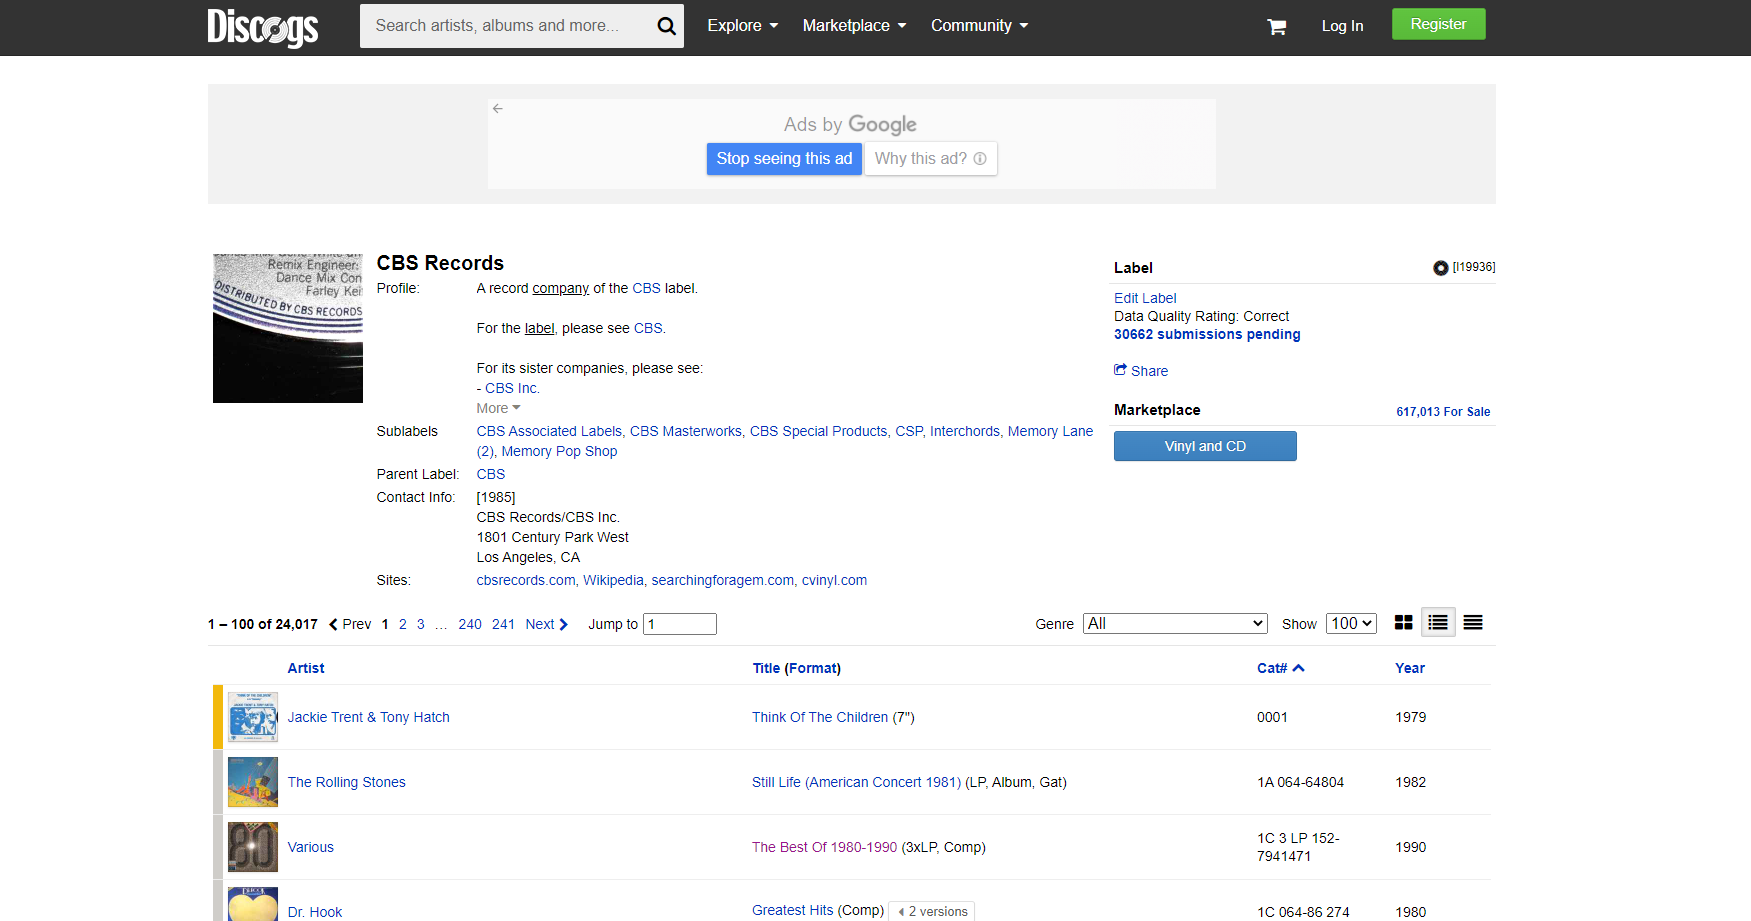
\includegraphics[width=0.75\textwidth,frame]{4221-t7/cbs_record.png}
	\end{figure}\vspace{-10pt}
\end{frame}

\begin{frame}[fragile]{Question 1 Cont.}
	
\textbf{Solution:}

\begin{lstlisting}[style=xml-small]
<album>
	<title></title>
	<artists>
		<artist></artist>
	</artists>
	<songs>
		<song>
			<title></title>
			<duration></duration>
		</song>
	</songs>
	<genres>
		<genre></genre>
	</genres>
	<year></year>
</album>
\end{lstlisting}
\end{frame}

\section*{Question 2 DTD}
\begin{frame}[fragile]{Question 2 DTD}

\textbf{Q2.1} Add an internal DTD for the XML document above. Make the DTD as tight as possible.

\textbf{Solution:}

\begin{lstlisting}[style=xml-small]
<?xml version="1.0" encoding="UTF-8"?>
<!DOCTYPE library [
	<!ELEMENT library (album*)>
	<!ELEMENT album (title,artists,songs,genres,year)>
	<!ELEMENT artists (artist*)>
	<!ELEMENT genres (genre*)>
	<!ELEMENT songs (song+)>
	<!ELEMENT artist (name,country)>
	<!ELEMENT song (title,duration)>
	<!ELEMENT title (#PCDATA)>
	<!ELEMENT name (#PCDATA)>
	<!ELEMENT country (#PCDATA)>
	<!ELEMENT duration (#PCDATA)>
	<!ELEMENT genre (#PCDATA)>
	<!ELEMENT year (#PCDATA)>
]>
<library>
	... <!-- Place your library data here -->
</library>
\end{lstlisting}
\end{frame}

\begin{frame}[fragile]{Question 2}
\begin{block}{DTD Syntax}
Note that \textbf{``*'' means zero or more}, \textbf{``+'' means one or more} and \textbf{no sign after the text means exactly one}. 
Of these, exactly one is of course the most tight but not necessarily possible for the document we are working with. \\
\textbf{\#PCDATA} is parsed character data, which we for this module essentially can think of as where we store raw values, i.e., values that do not consist of sub elements.
\end{block}	

\textbf{Q2.2} Validate the XML document with its DTD using eXist-db. Try to change the structure of the document so it is invalid and observe the error messages generated by eXist-db.
\begin{block}{}
	This is an open question based on the DTD defined. E.g., you may try to remove the \textbf{year} attribute from one \textbf{album}. You can also try with multiple \textbf{country} attributes in one \textbf{artist}.
\end{block}	
\end{frame}


\section*{Question 3 XPath}

\begin{frame}[fragile]{Question 3}
Translate the following queries into XPath.\\\vspace{5pt}
Your answers to the questions should include an XPath query with complete path as well as one with a more concise
path, where relevant. Your answers to the questions should include an XPath query with the full syntax and as
well as one using the shorthand syntax.\\\vspace{5pt}
Evaluate the queries using eXist-db. eXist-db only shows 10 elements by default. You should wrap your query in
an outer element to easily see all elements, i.e. \texttt{<results>\{ XPath query \}</results>}. For brevity, the solutions
are shown without this wrapping.\\\vspace{5pt}
\end{frame}

\begin{frame}[fragile]{Question 3.1 (Simple Query Expressions)}
Find the title of the songs.\\ \vspace{5pt}

\textbf{Solution}: \\
Let's try to find a answer with the explicit axes first (not the descendant::shorthand)
\begin{lstlisting}[style=xml-small-nomargin]
doc("library.xml")/child::library/child::album/child::songs/child::song/child::title
\end{lstlisting}\vspace{5pt}
...or, equivalently with the descendant,
\begin{lstlisting}[style=xml-small-nomargin]
doc("library.xml")/descendant::song/child::title
\end{lstlisting}\vspace{5pt}

By applying shorthand, we can query as follows:
\begin{lstlisting}[style=xml-small-nomargin]
doc("library.xml")/library/album/songs/song/title
\end{lstlisting}

\begin{lstlisting}[style=xml-small-nomargin]
doc("library.xml")//song/title
\end{lstlisting}\vspace{5pt}
\end{frame}


\begin{frame}[fragile]{Question 3.1 Cont.}
The query below does not work and gives the wrong result. (Why?)\\ \vspace{5pt}
\begin{lstlisting}[style=xml-small-nomargin]
doc("library.xml")/descendant::title
\end{lstlisting}

\begin{figure}
	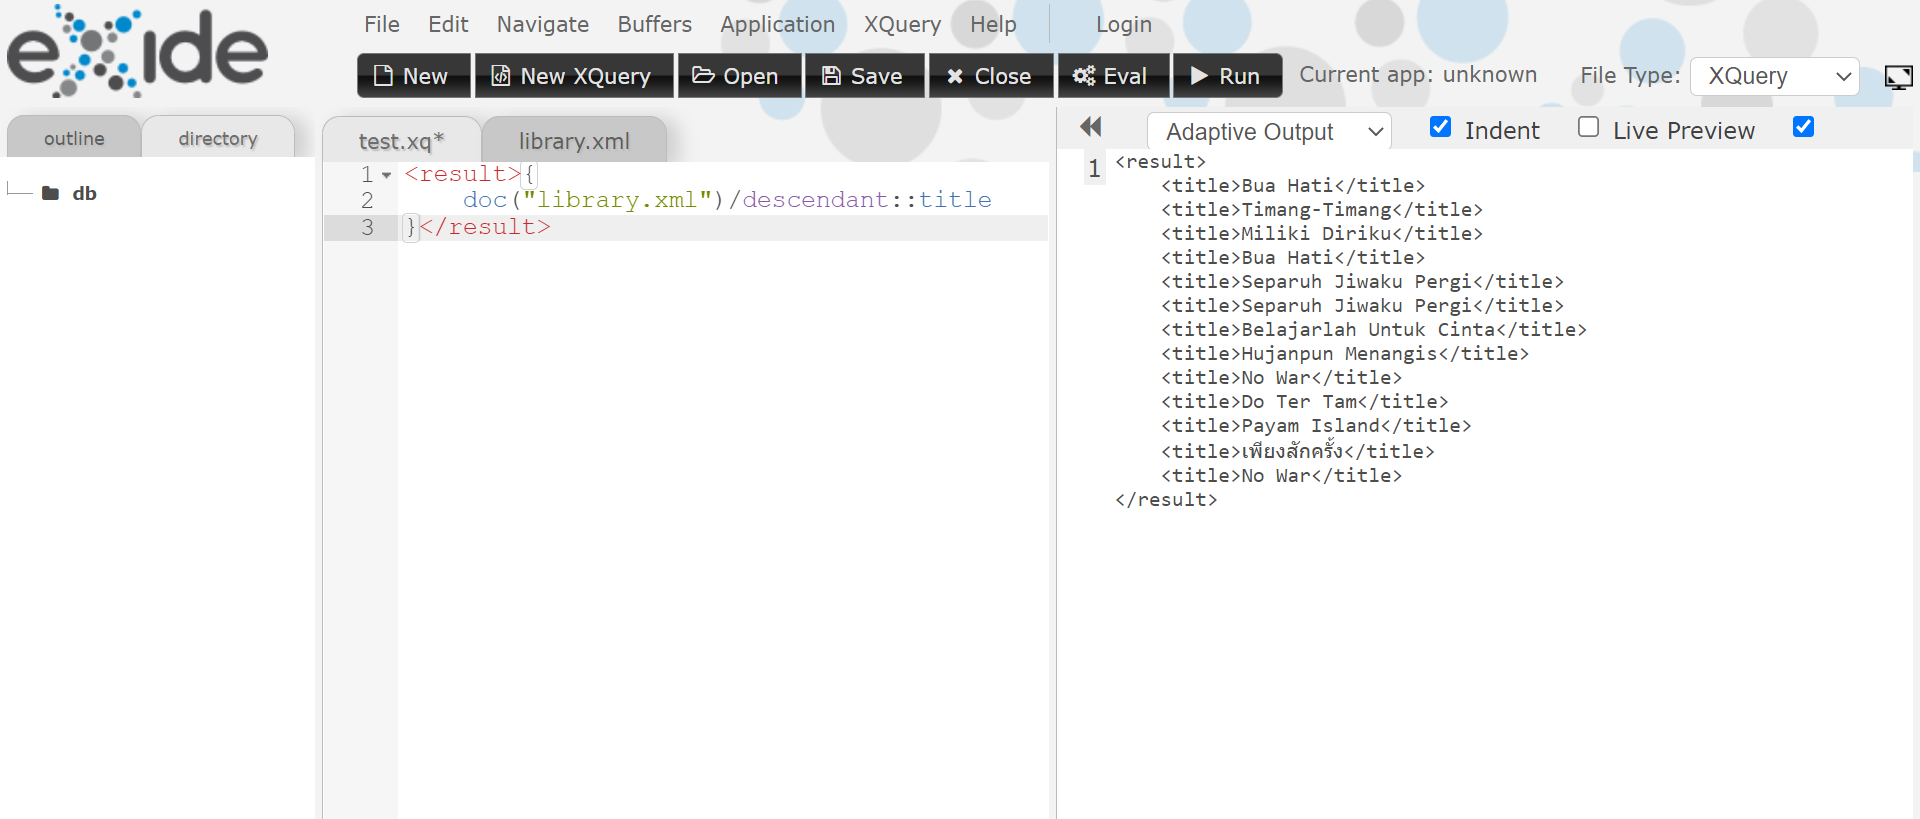
\includegraphics[width=0.95\textwidth,frame]{4221-t7/q3_1_wrong_result.png}
	\caption{Output of the eXide (without adding extra albums from CBS)}
\end{figure}\vspace{-10pt}
\end{frame}
	
\begin{frame}[fragile]{Question 3.2 (Filter Expression)}
Find the names of the Indonesian artists interpreting songs published between 1990 and 2000.

\textbf{Solution}: \\
(Query expression with the descendant)
\begin{lstlisting}[style=xml-small-nomargin]
doc("library.xml")/descendant::album[child::year>=1990 and child::year <=2000]
/child::artists/child::artist[child::country='Indonesia']/child::name
\end{lstlisting}\vspace{5pt}
...or, equivalently,
\begin{lstlisting}[style=xml-small-nomargin]
doc("library.xml")//album[year>=1990 and year <=2000]/artists/artist[country='Indonesia']/name
\end{lstlisting}\vspace{5pt}

\begin{block}{To read more...}
	Documentation: \url{https://exist-db.org/exist/apps/doc/newrangeindex}
\end{block}
\end{frame}

\begin{frame}[fragile]{Question 3.3 \& 3.4 (Count Clause)}
Find how many songs in the library were interpreted by Anang Ashanty.\\\vspace{5pt}
	
\textbf{Solution}: \\
\begin{lstlisting}[style=xml-small-nomargin]
count(doc("library.xml")/child::library/child::album[child::artists/child::artist/child::name='Anang Ashanty']/child::songs/child::song)
\end{lstlisting}\vspace{5pt}
...or, equivalently,
\begin{lstlisting}[style=xml-small-nomargin]
count(doc("library.xml")/library/album[artists/artist/name='Anang Ashanty']/songs/song)
<!-- the most concise form is shown below -->
count(doc("library.xml")//album[artists//name='Anang Ashanty']//song)
\end{lstlisting}\vspace{5pt}

\textbf{Caution}:
\begin{lstlisting}[style=xml-small-nomargin]
count(doc("library.xml")//album[//name='Anang Ashanty']//song)
\end{lstlisting}
The expression above does not work because the condition inside [\ ] became uncorrelated to node.

\end{frame}

\begin{frame}[fragile]{Question 3.3 \& 3.4 Cont.}
Find the title of the albums in the library with four songs or more.\\\vspace{5pt}
	
\textbf{Solution}: \\
\begin{lstlisting}[style=xml-small-nomargin]
doc("library.xml")/child::library/child::album[count(child::songs/child::song)>=4]/child::title
\end{lstlisting}\vspace{5pt}
...or, equivalently,
\begin{lstlisting}[style=xml-small-nomargin]
doc("library.xml")/library/album[count(songs/song)>=4]/title
\end{lstlisting}\vspace{5pt}

\end{frame}


\begin{frame}[fragile]{Question 3.5 (Axes)}
Propose an interesting query that uses different axes than ``child'' and ``descendant''. Write the query in English and in XPath.\\\vspace{10pt}
\textbf{Solution}: \\
For example we may use \texttt{ancestor} to query all albums' titles that have include songs performed by the artist Anang Ashanty.
\begin{lstlisting}[style=xml-small-nomargin]
doc("library.xml")/child::library/child::album/child::artists[child::artist/child::name='Anang Ashanty']/ancestor::album/child::title
\end{lstlisting}\vspace{5pt}

\begin{block}{To read more...}
	Documentation: \url{https://exist-db.org/exist/apps/doc/xquery} \\
	($\mathsection$ Current Status of XQuery Support $\rightarrow$ Supported Optional Features)
\end{block}	
\end{frame}

\begin{frame}{}
	\centering  
	For any further question, please feel free to email me:\vspace{10pt}
	
	huasong.meng@u.nus.edu \vspace{20pt}
	
	\begin{tcolorbox}
		\begin{center}
			\textcolor{red}{Copyright 2021 Mark H. Meng. All rights reserved.}
		\end{center}
	\end{tcolorbox}
\end{frame}